\documentclass{beamer}

\mode<presentation>
{
   \usetheme{EEng}
  \setbeamercovered{transparent}
  \setbeamercolor{background canvas}{bg=black!0}
}

\usepackage{enumerate}
\usepackage{array}
\usepackage{pifont} % for \cross symbol newcommand
\usepackage{graphics}
\usepackage{graphicx}
\usepackage{ucs}
\usepackage[utf8x]{inputenc}
\usepackage[english]{babel}
\usepackage{amsmath, amsthm, amssymb}
\usepackage[caption=false,font=footnotesize]{subfig}
\usepackage{amsmath}
\usepackage{amsfonts}
\usepackage{url}
\usepackage{listings}
\usepackage{color}

\newcommand{\checkK}{\color{green}\checkmark}
\newcommand{\cross}{\color{red}\hspace{-3pt}\ding{55}}
\newcommand{\bigexclaim}{\color{Dandelion}$\bigtriangleup$\hspace{-5.6pt}!}
\lstdefinelanguage{codeTTN}
{
        basicstyle=\ttfamily\tiny,
        sensitive=true,
        showstringspaces=false,
        numberblanklines=true,
        showspaces=false,
        breaklines=true,
        showtabs=false,
		numbers=left,
		numberstyle=\tiny,
		xleftmargin=15pt,
}
\lstnewenvironment{code}{\lstset{language=codeTTN}}{}

\title{Automatic Test Generation for Space}
\author{Ulisses Costa \and Daniela da Cruz \and Pedro Rangel Henriques}
\institute{SLATE'12 - Symposium on Languages, Applications and Technologies}
\date{\today}

\begin{document}
\begin{frame}
   \titlepage
\end{frame}

\begin{frame}\frametitle{Context}
\begin{block}{Problem}
VST (Visionspace Technologies) provides services related to testing for ESA and want to automate
the test generation for the Operational Simulator platform.
\end{block}

A tese de mestrado, no âmbito da qual esta apresentação se enquadra tem como objectivos:
\begin{itemize}
\item Gerar testes de forma automática para \textit{Operational Simulator}
\item Gerar testes unitários para a linguagem em que o \textit{Operational Simulator} está escrito, C++
\item Parametrizar o tamanho das estruturas de dados geradas e outros atributos
\end{itemize}
\end{frame}

\begin{frame}\frametitle{Motivação}
Proposta:
\begin{itemize}
\item Extrair UML e OCL a partir do código
\item Extrair testes a partir do código
\end{itemize}
\end{frame}

\begin{frame}\frametitle{Inferir OCL}
OCL é uma linguagem para descrever propriedades lógicas sobre modelos UML, tipicamente na forma de invariantes que tem de ser respeitados durante todo o tempo de execução.\\

Numa primeira fase é importante abstrair da implementação para descobrir "regras" a mas alto nível.
\begin{itemize}
\item Gerar diagrama de UML para o código existente (fácil)
\item Inferir Invariantes do código (difícil)
\item Relacionar os Invariantes descobertos com os diagramas
\end{itemize}
\end{frame}

\begin{frame}\frametitle{White vs. Black Box Testing}
\begin{block}{Tipos de testes relativamente ao conhecimento do código}
\begin{description}
\item[White Box], há conhecimento do código fonte e este é usado para a tarefa de teste.
\item[Black Box], há conhecimento apenas dos requisitos funcionais do código e de como cada componente do código deverá comportar-se.
\end{description}
\end{block}
\end{frame}

\begin{frame}\frametitle{Abordagens 1/2}
\begin{description}
\item[Specification-based Generation Testing], \textit{aka Model Based Testing} consiste em testar um programa baseando-se na especificação ou no modelo do programa.
Em especifico pode-se gerar uma bateria de casos para teste diretamente a partir da especificação do comportamento do programa, sem considerar o código do programa.
\end{description}
\end{frame}

\begin{frame}\frametitle{Abordagens 2/2}
\begin{description}
\item[Constraint-based Generation Testing], pode ser usado para seleccionar baterias de casos para teste que satisfaçam restrições sobre um conjunto de variaveis.
Quando combinado com execução simbólica, coleccta restrições ao longo dos diferentes caminhos no \textit{CFG}.
Posteriormente é possivel resolver estas restrições e produzir baterias de casos para teste a partir daí.
\end{description}
Outras foram estudadas, para mais informação consultar o paper.
\end{frame}

\begin{frame}\frametitle{Estado actual}
Até agora foram estudadas várias ferramentas, as mais importantes e mais desenvolvidas:
\begin{itemize}
\item Korat, é uma framework madura para construir automaticamente estruturas complexas em JAVA
\item Pex, é uma ferramenta automatica da Microsoft de \textit{White-box testing} que garante cobertura total
\end{itemize}
\end{frame}

\begin{frame}[fragile] \frametitle{Ferramentas Estudadas - Pex}
\begin{code}
public class Program {
  public static int BSearch(int x, int n) {
    return BinarySearch(x, 0, n);
  }
  static int BinarySearch(int x, int lo, int hi) {
    while (lo < hi) {
      int mid = (lo+hi)/2;
      Debug.Assert(mid >= lo && mid < hi);
      if (x < mid) { hi = mid; } else { lo = mid+1; }
    }
    return lo;
  }
}
\end{code}

{\tiny \begin{tabular}{|c|c|c|c|c|}\hline
Result & x & n & result & Output/Exception \\\hline
\checkK & 0 & 0 & 0      & \\\hline
\checkK & 0 & 1 & 1      & \\\hline
\checkK & 0 & 3 & 1      & \\\hline
\cross & 1073741888 & 1719676992 & & TraceAssertionException \\\hline
\checkK & 1 & 6 & 2      & \\\hline
\checkK & 50 & 96 & 51      &\\\hline
\end{tabular}
}
\end{frame}

\def\t#1#2#3#4{\langle#1 \ #2 : #3 \ : #4 \ \rangle}
\def\d#1#2#3{\langle#1 \ #2 :: #3 \ \rangle}
\newcommand{\subseteqL}{\mathbin{\subseteq\mkern-4mu\subseteq}}
\newcommand{\inL}{\mathbin{\in\mkern-4mu\in}}

\begin{frame}[fragile]\frametitle{Ferramentas Estudadas - Korat}
\begin{code}
public class LinkedList<T> {
  public static class LinkedListElement<T> {
    public T Data;
    public LinkedListElement<T> Prev;
    public LinkedListElement<T> Next;
  }
  private LinkedListElement<T> Head;
  private LinkedListElement<T> Tail;
  private int size; 
}
\end{code}
Invariantes da classe $LinkedList$ (lista duplamente ligada circular):
{\tiny
\begin{eqnarray}
\t \forall {l} {l \in LinkedList} {Head(l) \equiv null \vee Tail(l) \equiv null \Leftrightarrow size(l) \equiv 0}\\
\t \forall {l} {l \in LinkedList} {Tail(l).Next \equiv null}\\
\t \forall {l} {l \in LinkedList} {Head(l).Prev \equiv null}\\
\t \forall {l} {l \in LinkedList} {size(l) \equiv 1 \Leftrightarrow Head(l) \equiv Tail(l)}\\
\t \forall {l} {l \in LinkedList} {\t \forall {e_1,e_2} {\{e_1,e_2\} \subseteqL l} {\t \exists {e} {e \inL l} {e_1.Next \equiv e \wedge e_2.Prev \equiv e}}\label{eq:linked}}\\
\t \forall {l} {l \in LinkedList} {\t \forall {e_1,e_2} {\{e_1,e_2\} \subseteqL l} {e_1 \equiv e_2 \Rightarrow i(e_1) \equiv i(e_2)}\label{eq:uniq}}
\end{eqnarray}
}
\end{frame}

\begin{frame}[fragile]\frametitle{Ferramentas Estudadas - Pex - $LinkedList$}
\begin{figure}[!ht]
\centerline{
\subfloat[Instância de $LinkedList$ instance gerada pelo pex para testar o método $Remove$]{
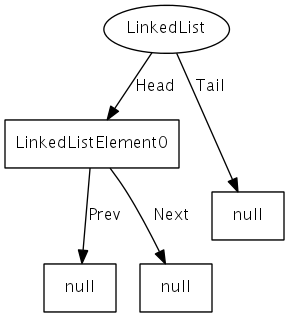
\includegraphics[width=.3\textwidth]{img/pex1}
}
\hfil
\subfloat[Instância de $LinkedList$ instance gerada pelo pex para testar o método $Find$]{
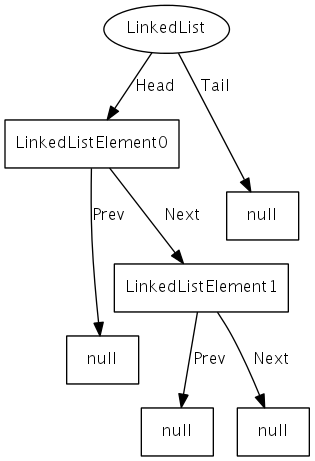
\includegraphics[width=.3\textwidth]{img/pex2}
\label{fig:pexinst2}}}
\caption{Exemplos de instâncias geradas pelo pex para a classe $LinkedList$.}
\label{fig:pexG}
\end{figure}
\end{frame}

\begin{frame}[fragile]\frametitle{Ferramentas Estudadas - Korat - $LinkedList$}
\begin{figure}[!ht]
\centerline{
\subfloat[Instância de $LinkedList$ com $2$ elementos]{
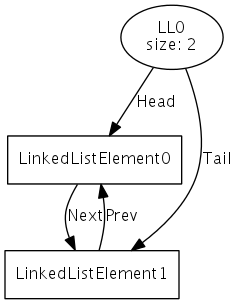
\includegraphics[width=.2\textwidth]{img/ll1}
}
\hfil
\subfloat[Instância de $LinkedList$ com $5$ elementos]{
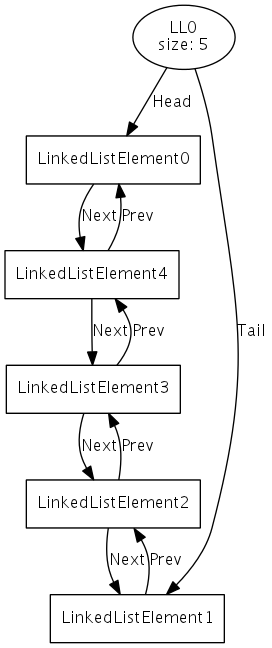
\includegraphics[width=.2\textwidth]{img/ll2}
}}
\end{figure}
\end{frame}

\begin{frame}[fragile]\frametitle{Ferramentas Estudadas - Sumário}
\begin{block}{Sumário}
O Pex usa análise estática e é muito eficiente em descobrir todos os caminhos de execução possíveis em métodos C\#.
O Pex tambem pode ser utilizado para gerar testcases das classes, mas as instâncias geradas não mantém os invariantes das estruturas de dados.\\

Por outro lado o Korat é a ferramenta ideal para a tarefa de gerar estruturas que cumpram os invariantes pedidos.
\end{block}
\end{frame}

\begin{frame} \frametitle{Conclusão e Trabalho Futuro}
\begin{itemize}
\item Pex provou ser uma ferramenta poderosa a dar cobertura total
\item Korat mostrou ser uma ferramenta muito útil para gerar estruturas complexas
\end{itemize}
A mistura entre a análise estática do Pex com a capacidade de gerar estruturas úteis do Korat é o caminho que vamos seguir.\\

Será estudado a inferência de pre- pos condições e invariantes[Moy 2009] para conseguir inferir OCL.
\end{frame}

\begin{frame}[fragile] \frametitle{Método $repOK$ do Korat para $LinkedList$}
\begin{code}
public boolean repOK() {
  if(Head == null || Tail == null)
    return size == 0;
  if(size == 1) return Head == Tail;
  if(Head.Prev != null) return false;
  if(Tail.Next != null) return false;
  LinkedListElement<T> last = Head;
  Set visited = new HashSet();
  LinkedList workList = new LinkedList();
  visited.add(Head);
  workList.add(Head);
  while (!workList.isEmpty()) {
    LinkedListElement<T> current = (LinkedListElement<T>) workList.removeFirst();
    if (current.Next != null) {
      if (!visited.add(current.Next))
	    return false;
      workList.add(current.Next);
      if(current.Next.Prev != current) return false;
      last = current.Next;
    }
  }
  if(last != Tail)
    return false;
  return (visited.size() == size);
}
\end{code}
\end{frame}

\end{document}

